% Created 2014-07-09 Wed 03:46
\documentclass[utf8x,notes,17pt]{beamer}
\usepackage[utf8]{inputenc}
\usepackage[T1]{fontenc}
\usepackage{fixltx2e}
\usepackage{graphicx}
\usepackage{longtable}
\usepackage{float}
\usepackage{wrapfig}
\usepackage{rotating}
\usepackage[normalem]{ulem}
\usepackage{amsmath}
\usepackage{textcomp}
\usepackage{marvosym}
\usepackage{wasysym}
\usepackage{amssymb}
\usepackage{hyperref}
\tolerance=1000
\setbeamertemplate{navigation symbols}{}
\usepackage{courier}
\usepackage{helvet}
\usepackage{listings}
\usepackage{pdfcomment}
\SetUnicodeOption{mathletters}
\DeclareUnicodeCharacter{952}{\theta}
\lstset{
keywordstyle=\color{blue}
, basicstyle=\ttfamily\small
, commentstyle={}
, columns=fullflexible
, showstringspaces=false
, keepspaces=false
, breaklines=true
}
\newcommand{\head}[1]{\begin{center}
\vspace{13mm}\hspace{-1mm}\Huge{{#1}}
\end{center}}
\renewcommand{\note}[1]{\marginnote{\pdfcomment[icon=note]{#1}}}
\usetheme[height=16mm]{Rochester}
\author{John Wiegley}
\date{4 Jul 2014}
\title{Monads and other abstractions}
\hypersetup{
  pdfkeywords={math monad haskell functional programming},
  pdfsubject={Applying mathematical abstractions to functional programming},
  pdfcreator={Emacs 24.3.1 (Org mode 8.2.6)}}
\begin{document}

\maketitle
\setbeamertemplate{footline}{}
\setbeamerfont{block body}{size=\small}
\setbeamercolor{bgcolor}{fg=white,bg=blue}

\section{Mathematics}
\label{sec-1}
\begin{frame}[fragile,plain,label=sec-1-1]{HEAD}
\head{Mathematics}
\end{frame}
\begin{frame}[fragile,label=sec-1-2]{Meaning}
There isn't any.
\note{note
This is just some notes.}
\end{frame}
\begin{frame}[fragile,label=sec-1-3]{Abstraction}
Structures, and relationships between structures.
\end{frame}
\section{Sets}
\label{sec-2}
\begin{frame}[fragile,plain,label=sec-2-1]{HEAD}
\head{Sets}
\note{note
What is really interesting is just how much can be done with such a minimal
amount of structure.}
\end{frame}
\begin{frame}[fragile,label=sec-2-2]{``Stuff''}
A set is a collection of elements.
\begin{example}<2->[\vspace*{-3.5ex}]%x
\begin{lstlisting}[language=Haskell]
type Set a = a -> Bool
\end{lstlisting}
\end{example}
\end{frame}
\begin{frame}[fragile,label=sec-2-3]{Extensional}
Can be defined by stating its elements.
\begin{example}[\vspace*{-3.5ex}]%x
\( \{ \ True, False\ \} \)
\end{example}
\end{frame}
\begin{frame}[fragile,label=sec-2-4]{Intensional}
Or by describing them.
\begin{example}[\vspace*{-3.5ex}]%x
\( \{ \ x \ |\  x \in \mathbb{N}, even(x)\ \} \)
\end{example}
\end{frame}
\begin{frame}[fragile,label=sec-2-5]{Distinction}
Values can be extensionally equal, but intensionally distinct.
\begin{example}[\vspace*{-3.5ex}]%x
\( n ↦ 2 (n + 5) \)

\( n ↦ 2 n + 10 \)
\end{example}
\end{frame}
\begin{frame}[fragile,label=sec-2-6]{Deceptively simple}
With just a definition of sets, and seven axioms (and we've already seen
two!), you can generate a good part of mathematics.
\end{frame}
\section{Functions}
\label{sec-3}
\begin{frame}[fragile,plain,label=sec-3-1]{HEAD}
\head{Functions}
\end{frame}
\begin{frame}[fragile,label=sec-3-2]{As maps}
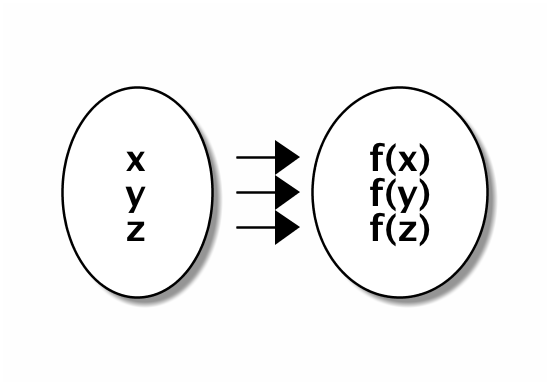
\includegraphics[width=.9\linewidth]{maps.png}
\end{frame}
\begin{frame}[fragile,label=sec-3-3]{Higher-order functions}
\[ id\ x = x \]

\[ (f ∘ g)\ x = f (g(x)) \]
\end{frame}
\begin{frame}[fragile,label=sec-3-4]{Properties of functions}
\[ f : cod → dom \]
\note{note
A powerful concept is to define properties of functions in terms of functions
and equalities.}
\begin{definition}<2->[Idempotent]%x
\( f ∘ f = f \)
\end{definition}
\begin{definition}<3->[Involutive]%x
\( f ∘ f = id \)
\end{definition}
\end{frame}
\begin{frame}[fragile,label=sec-3-5]{Homomorphism}
``Structure preserving.''
\end{frame}
\begin{frame}[fragile,label=sec-3-6]{Isomorphism}
An isomorphism is a pair of functions satisfying two equations:

\[ f ∘ g = id_{dom(f)} \]
\[ g ∘ f = id_{dom(g)} \]
\end{frame}
\begin{frame}[fragile,label=sec-3-7]{Isomorphism}
In terms of the types involved:

\[ A ≅ B \]

\[ g : A → B \]
\[ f : B → A \]
\note{note
Assuming of course \( dom(f) = A, dom(g) = B \).}
\end{frame}
\section{Laws}
\label{sec-4}
\begin{frame}[fragile,plain,label=sec-4-1]{HEAD}
\head{Laws}
\end{frame}
\section{Algebras}
\label{sec-5}
\begin{frame}[fragile,plain,label=sec-5-1]{HEAD}
\head{Algebras}
\end{frame}
\section{Algebraic Structures}
\label{sec-6}
\begin{frame}[fragile,plain,label=sec-6-1]{HEAD}
\head{Algebraic Structures}
\end{frame}
\begin{frame}[fragile,label=sec-6-2]{Magmas}
\end{frame}
\begin{frame}[fragile,label=sec-6-3]{Semigroups}
\end{frame}
\begin{frame}[fragile,label=sec-6-4]{Monoids}
\end{frame}
\begin{frame}[fragile,label=sec-6-5]{Groups}
\end{frame}
\section{Type Algebras}
\label{sec-7}
\begin{frame}[fragile,plain,label=sec-7-1]{HEAD}
\head{Type Algebras}
\end{frame}
\section{Equational Reasoning}
\label{sec-8}
\begin{frame}[fragile,plain,label=sec-8-1]{HEAD}
\head{Equational Reasoning}
\end{frame}
\section{Quantification}
\label{sec-9}
\begin{frame}[fragile,plain,label=sec-9-1]{HEAD}
\head{Quantification}
\end{frame}
\begin{frame}[fragile,label=sec-9-2]{Existential}
\[ \exists p, P(p) \]
\end{frame}
\begin{frame}[fragile,label=sec-9-3]{Universal}
\[ \forall p, P(p) \]
\end{frame}
\begin{frame}[fragile,label=sec-9-4]{Universal}
\begin{alertblock}{True?}%x
$\forall$ x, $\exists$ y $\rightarrow$ x = y
\end{alertblock}
\end{frame}
\begin{frame}[fragile,label=sec-9-5]{Universal}
\begin{alertblock}{True?}%x
$\forall$ x, $\exists$ y $\rightarrow$ x $\neq$ y
\end{alertblock}
\end{frame}
\section{Parametricity}
\label{sec-10}
\begin{frame}[fragile,plain,label=sec-10-1]{HEAD}
\head{Parametricity}
\end{frame}
\section{Curry-Howard Isomorphism}
\label{sec-11}
\begin{frame}[fragile,plain,label=sec-11-1]{HEAD}
\head{Curry-Howard Isomorphism}
\end{frame}
\section{Free objects}
\label{sec-12}
\begin{frame}[fragile,plain,label=sec-12-1]{HEAD}
\head{Free objects}
\end{frame}
\section{Category Theory}
\label{sec-13}
\begin{frame}[fragile,plain,label=sec-13-1]{HEAD}
\head{Category Theory}
\end{frame}
\section{Functors}
\label{sec-14}
\begin{frame}[fragile,plain,label=sec-14-1]{HEAD}
\head{Functors}
\end{frame}
\section{Applicatives}
\label{sec-15}
\begin{frame}[fragile,plain,label=sec-15-1]{HEAD}
\head{Applicatives}
\end{frame}
\section{Monads}
\label{sec-16}
\begin{frame}[fragile,plain,label=sec-16-1]{HEAD}
\head{Monads}
\end{frame}
\section{Free Monads}
\label{sec-17}
\begin{frame}[fragile,plain,label=sec-17-1]{HEAD}
\head{Free Monads}
\end{frame}
\section{Colophon}
\label{sec-18}
% Emacs 24.3.1 (Org mode 8.2.6)
\end{document}